% Author: Izaak Neutelings (Februari, 2020)
% page 8 https://archive.org/details/StaticAndDynamicElectricity
% https://tex.stackexchange.com/questions/56353/extract-x-y-coordinate-of-an-arbitrary-point-on-curve-in-tikz
% https://tex.stackexchange.com/questions/412899/tikz-calculate-and-store-the-euclidian-distance-between-two-coordinates

\documentclass[border=3pt,tikz]{standalone}
\usepackage{amsmath} % for \dfrac
\usepackage{bm}
\usepackage{physics}
\usepackage{tikz,pgfplots}
\usepackage[outline]{contour} % glow around text
\usetikzlibrary{angles,quotes} % for pic (angle labels)
\usetikzlibrary{decorations.markings}
\usetikzlibrary{shapes,intersections} % for path name
\tikzset{>=latex} % for LaTeX arrow head
\contourlength{1.8pt}

\usepackage{xcolor}
\colorlet{Ecol}{orange!90!black}
\colorlet{EcolFL}{orange!80!black}
\colorlet{veccol}{green!45!black}
\colorlet{EFcol}{red!60!black}
\colorlet{pluscol}{red!60!black}
\colorlet{minuscol}{blue!60!black}
\colorlet{gausscol}{green!50!black!80}
\tikzstyle{charged}=[top color=blue!20,bottom color=blue!40,shading angle=10]
\tikzstyle{charge+}=[very thin,draw=black,top color=red!80,bottom color=red!80!black,shading angle=-5]
\tikzstyle{charge-}=[very thin,draw=black,top color=blue!50,bottom color=blue!70!white!90!black,shading angle=10]
\tikzstyle{darkcharged}=[very thin,top color=blue!60,bottom color=blue!80,shading angle=10]
\tikzstyle{gauss surf}=[green!40!black,top color=green!2,bottom color=green!80!black!70,shading angle=5,fill opacity=0.6]
\tikzstyle{gauss dark}=[green!40!black,fill=green!40!black!70,fill opacity=0.8]
\tikzstyle{gauss line}=[green!40!black]
\tikzstyle{gauss dashed line}=[green!60!black!80,dashed,line width=0.2]
\tikzstyle{vector}=[->,thick,veccol]
\tikzstyle{normalvec}=[->,thick,blue!80!black!80]
\tikzstyle{EField}=[->,thick,Ecol]
\tikzstyle{EField dashed}=[dashed,Ecol,line width=0.6]
\tikzset{
  EFieldLine/.style={thick,EcolFL,decoration={markings,
                     mark=at position #1 with {\arrow{latex}}},
                     postaction={decorate}},
  EFieldLine/.default=0.5}
\tikzstyle{metal}=[top color=black!5,bottom color=black!15,shading angle=30]
\tikzstyle{measure}=[fill=green!70!black!8,midway,outer sep=0,inner sep=1]
\def\L{2.2}
\def\H{2.2}
\def\W{0.30}
\def\Nx{5}
\def\Ny{5}

%\pgfdeclareradialshading{myball}{\pgfpoint{0.5cm}{0cm}}% 
%  {rgb(0cm)=(1,1,1); rgb(0.7cm)=(0.7,0.1,0); rgb(1cm)=(0.5,0.05,0); rgb(1.05cm)=(1,1,1)}


\begin{document}


% SOLID CHARGED SPHERE 3D
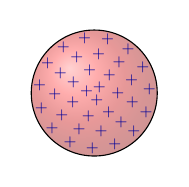
\begin{tikzpicture}
  \def\NQ{4} %13}
  \def\NE{7}
  \def\R{1}
  \def\r{2.6}
  \def\dtheta{50}
  \def\angle{135}
  \coordinate (P) at (\angle:0.83*\r);
  
  % SPHERE
  % \draw[gauss line,ball color=green!70!black,fill opacity=0.3]
    % (0,0) circle (\r);

    % \def\larg{0.3}
    % \fill[gray,opacity=0.8,draw opacity=0] (0,-\R+0.25*\larg) -- ++ (0,2*\R) -- ++ (\larg,0.25*\larg) -- ++ (0,-2*\R) -- cycle;
 

  \fill[red!20]
    (0,0) circle (0.8*\R);
  \draw[ball color=red!80,fill opacity=0.3]
    (0,0) circle (0.8*\R);
  % \draw[<->,black,very thin]
    % (0,0) -- (-8:\R);
    %  node[pos=0.6,above=-1,black] {$R$};
  % \draw[vector]
    % (0,0) -- (P) node[pos=0.36,above=1] {$\vb{r}$};
  % \node at (-60:1.25*\R) {$Q = \rho V$};
  
  % CHARGES
  \foreach \i [evaluate={\rc=(\i-0.5)*0.8*\R/\NQ; \N=-1+4*\i;}] in {1,...,\NQ}{
    \foreach \j [evaluate={\ang=48+1*\i+\j*360/\N;}] in {1,...,\N}{
      \node[minuscol,scale=0.6] at (\ang:\rc) {$+$};
    }
  }
  % \def\larg{0.3}
  % \fill[gray,opacity=0.8,draw opacity=0,draw=black] (-\larg,-\R) -- ++ (0,2*\R) -- ++ (\larg,0.25*\larg) -- ++ (0,-2*\R) -- cycle;

  % \draw[] (+\larg,-\R+0.5*\larg+0.1) -- (+\larg,-\R+0.5*\larg) -- node[midway,below,black,opacity=1] {$\Pi$} (-\larg,-\R) -- ++ (0,2*\R) -- ++ (2*\larg,0.5*\larg) -- ++ (0,-0.4) ;
  
  
  % % FIELD LINES
  % \foreach \i [evaluate={\ang=10+\i*360/\NE;}] in {1,...,\NE}{
  %   \draw[EFieldLine=0.4] (\ang:\R) -- (\ang:1.2*\r);
  % }
  
  % % GAUSS FRONT
  % \draw[gauss line,ball color=green!70!black,fill opacity=0.2]
    % (0,\r) arc (90:270:\r) arc (180+\dtheta:180-\dtheta:{\r/sin(\dtheta)});
  
  % AREA ELEMENT
  % \draw[gauss dark,rotate=40] (P) ++ (\angle:0.015*\r) ellipse (0.2 and 0.1);
  % \draw[->,normalvec] (P) ++ (\angle-70:0.03*\r) --++ (\angle:0.25*\r) node[right=1,above] {$\vu{n}$};
  % \draw[->,EField] (P) ++ (\angle+70:0.03*\r) --++ (\angle:0.5*\r) node[left=1,above] {$\vb{E}$};
  
\end{tikzpicture}

\end{document}
